\section{Additional Strategy-Routing Diagnostics}
\label{app:strategy-diagnostics}

All quantities in this section are computed from the saved 29,520 worker
attempts.  Counterfactual allocations replay the same model--strategy traces
under a common twenty-retry horizon; they are not additional model calls.

\begin{figure}[H]
  \centering
  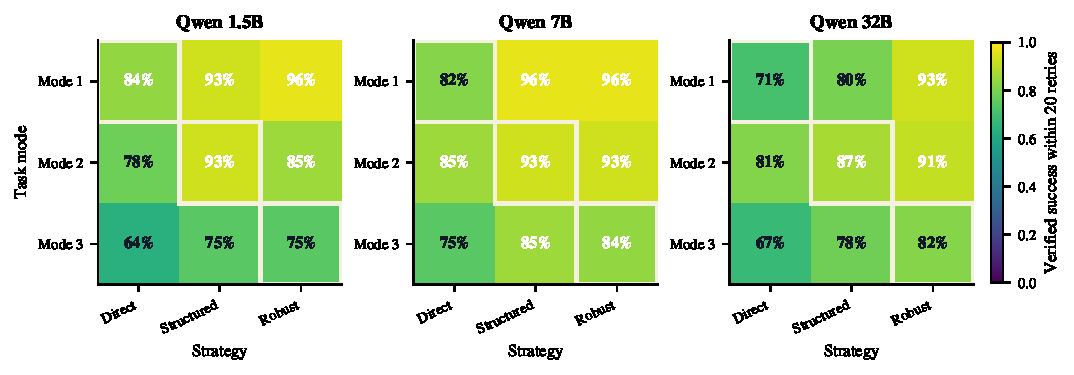
\includegraphics[width=0.88\textwidth]{figures/strategy_routing/strategy_specialization.pdf}
  \caption{\textbf{Mode-conditioned strategy specialization.}  Cells report
  verified success within twenty attempts.  Strategy performance varies with
  task mode and worker model, establishing the heterogeneity required for
  nontrivial allocation.}
  \label{fig:strategy-specialization}
\end{figure}

\begin{figure}[H]
  \centering
  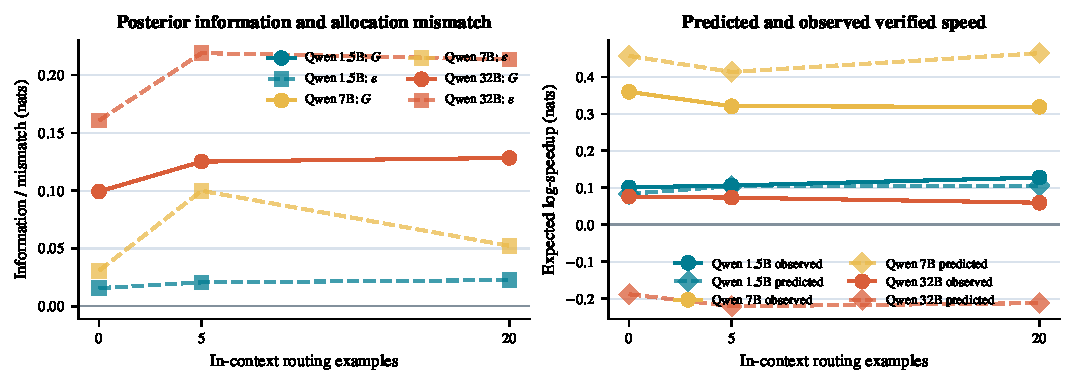
\includegraphics[width=0.92\textwidth]{figures/strategy_routing/information_speed_curve.pdf}
  \caption{\textbf{Information, mismatch, and packed speed.}  The left panel
  reports calibrated information and allocation mismatch as the number of
  in-context routing examples changes.  The right panel compares the resulting
  packed prediction with replayed packed log-speedup.}
  \label{fig:information-speed-curve}
\end{figure}

\begin{figure}[H]
  \centering
  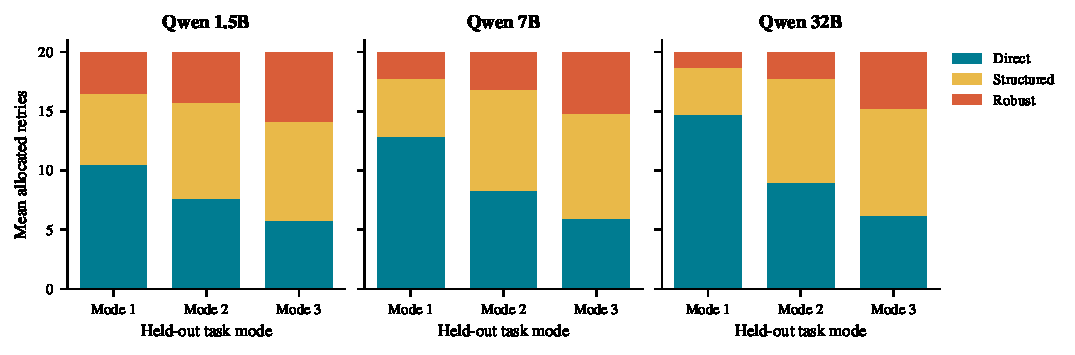
\includegraphics[width=0.80\textwidth]{figures/strategy_routing/router_allocations.pdf}
  \caption{\textbf{Mean strategy allocation by held-out task mode.}  Every bar
  contains exactly twenty retries.  The allocation changes with both task mode
  and worker model, while models and modes remain separate experimental
  objects.}
  \label{fig:router-allocations}
\end{figure}

\section{Theorem-to-Evidence Audit}
\label{app:theorem-evidence}

Exact identities are established by proof.  Experiments estimate their terms
and test their structural assumptions; they do not replace those proofs.

\begin{center}
\small
\renewcommand{\arraystretch}{1.2}
\begin{tabular}{@{}p{4.2cm}p{3.1cm}p{8.2cm}@{}}
\toprule
\textbf{Result} & \textbf{Status} & \textbf{Evidence and limitation} \\
\midrule
Posterior-matched allocation and Routing-Information Identity
& Partial
& Calibrated posteriors and realized strategy shares identify $G=0.128$ nat
and $\varepsilon=0.052$ nat for the reported 7B configuration.  The measured
inverse-share slopes, $0.661$ in seconds and $0.707$ in tokens, differ from the
ideal value~$1$. \\

Model-Aware Decomposition
& Partial
& The 1.5B-to-7B accounting estimates cost $0.008$, competence $0.381$,
information $0.128$, and mismatch $0.052$ nat.  Predicted and observed packed
gains differ by $-0.145$ nat. \\

Model-selection crossover
& Partial
& Mode--strategy cells have different cost--success profiles.  The experiment
does not statistically identify a globally optimal worker for every mode. \\

Single-mode retry crossover
& Partial
& Twenty repeated attempts estimate retry curves, but conditional i.i.d.
retries within each mode have not been established. \\

Paired allocation-gain estimator
& Protocol-aligned
& Router configuration is selected on validation data and evaluated once on 42
held-out tasks.  The solver-time comparison excludes router inference cost;
the measured batched cost is reported separately. \\

Approximate-packedness residual
& Partial
& The observed closure residual is finite, but a uniform bound
$|r_M|\le\eta$ over all admissible allocations is not established. \\
\bottomrule
\end{tabular}
\end{center}
